%\part{Probabilidad básica}

\section{Fundamentos de probabilidad}

\subsection{Experimentos aleatorios}

 \begin{exmp}
  \label{exmp:1.1}
  Si lanzamos una moneda, el resultado del experimento será ``águila'' (\emph{tail} en inglés) que simbolizaremos por $T$ o $0$ o ``sol''(\emph{head} en inglés) simbolizado por $H$ o $1$, es decir, uno de los elementos del conjunto $\set{T,H}$ (o bien $\set{0,1}.$)
 \end{exmp}



 \begin{exmp}
  \label{exmp:1.2}
  Si lanzamos un dado, el resultado del experimento resultará en uno de los números del conjunto $\set{1,2,3,4,5,6}.$
 \end{exmp}



 \begin{exmp}
  \label{exmp:1.3}
  Si lanzamos una moneda dos veces, existen cuatro posibles resultados:
  \begin{align*}
   \set{HH,HT,TH,TT}.
  \end{align*}

 \end{exmp}



 \begin{exmp}
  \label{exmp:1.4}
  Si estamos haciendo tornillos con una máquina, el resultado del experimento es que un tornillo puede salir defectuoso. Entonces cuando el tornillo este fabricado pertenecerá al conjunto
  \begin{align*}
   \set{\texttt{defectuoso, no defectuoso}}
  \end{align*}

 \end{exmp}



 \begin{exmp}
  \label{exmp:1.5}
  Si un experimento consiste en medir la \emph{vida útil} de una bombilla eléctrica producida por una compa\~nía, entonces el resultado del experimento es tiempo $t$ medido en horas en algún intervalo
  \begin{align*}
   0\leq t \leq T,
  \end{align*}
donde $T$ es el tiempo de vida máximo de una bombilla.
 \end{exmp}



\subsection{El espacio muestral}
{}
Un conjunto $S$ que consiste de todos los posibles resultados de un experimento aleatorio es llamado \emph{espacio muestral,}  y cada posible resultado es llamado un \emph{punto muestral.}

Usualmente existirá más de un espacio muestral que describe un experimento, pero usualmente, sólo uno provee la mayor información.

{}
\begin{exmp}
 \label{exmp:1.6}
 Si lanzamos un dado, un posible espacio muestral está dado por $\set{1,2,3,4,5,6},$  mientras que otro está dado por $\set{\text{par},\text{impar}}.$
\end{exmp}


{}
\begin{exmp}
 \label{exmp:1.7}
 Si lanzamos una moneda dos veces seguidas un posible espacio muestral esta dado en el ejemplo \ref{exmp:1.3},  mientras que otro esta dado por
 \begin{align*}
\set{(0,0), (0,1), (1,0),(1,1)}.
\end{align*}
\end{exmp}



\begin{figure}
 \centering
 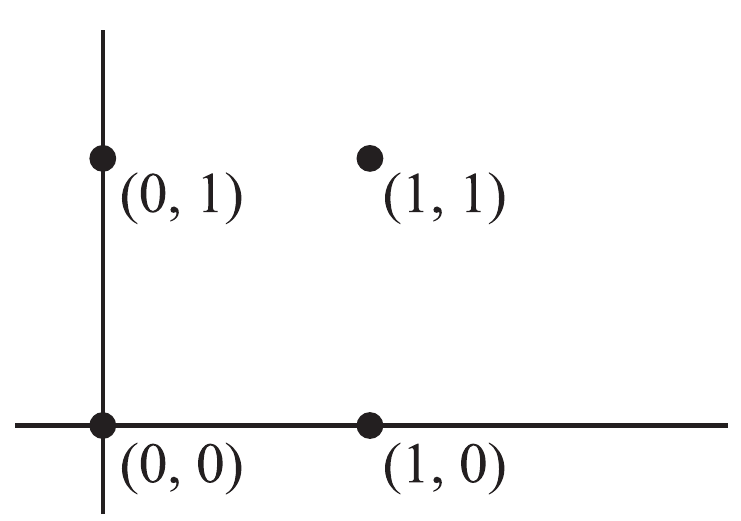
\includegraphics[width=5cm,keepaspectratio=true]{./pe/pands0101.png}
 % pands0101.png: 0x0 pixel, 300dpi, 0.00x0.00 cm, bb=
 \label{fig:0101}
\end{figure}


{Tipos de espacio muestral}
\begin{itemize}
 \item \emph{Finito:} tiene un número finito de puntos.
 \item \emph{Infinito numerable:} Tiene tantos puntos como los números naturales $\N$ (es decir, podemos numerar el espacio).
 \item \emph{Infinito no numerable:} Tiene tantos puntos como la recta real $\R.$  Por ejemplo, el intervalo $0<x<1.$
\end{itemize}


{}
Si el espacio muestral es finito o infinito numerable, diremos que es \emph{discreto.}  Si es infinito no numerable, diremos que es \emph{continuo.}

\subsection{Eventos}
{}
Un \emph{evento} es un subconjunto $A$ de un espacio muestral $S,$ es decir, un subconjunto de todos los posibles resultados de un experimento. 

Si el resultado es un elemento de $A,$ diremos que \emph{$A$ ha ocurrido.} 

Un evento que consiste de un único punto de $S$ es llamado a veces \emph{evento elemental o simple.}

{}
\begin{exmp}
 \label{exmp:1.8}
 Si lanzamos una moneda dos veces, el evento de que obtengamos \emph{exactamente} un águila  es un subconjunto del espacio muestral:
 
 \begin{figure}[h]
 \centering
 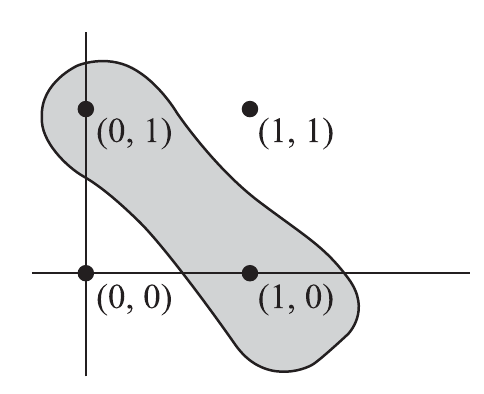
\includegraphics[height=3cm,keepaspectratio=true]{./pe/pands0102.png}
 % pands0102.png: 0x0 pixel, 300dpi, 0.00x0.00 cm, bb=
 \label{pands0102}
\end{figure}

\end{exmp}


{}
Como eventos particulares, podemos considerar todo el espacio muestral $S$ como el \emph{evento cierto o seguro} y el conjunto vacío $\emptyset$ como el \emph{evento imposible.}


{Operaciones entre eventos} Supongamos que $A,B$ son dos eventos. 
\begin{itemize}
 \item $A\cup B$ es el evento \texttt{``ocurre $A$ o $B$ o ambos'',} y también es llamado \emph{unión de $A$ con $B$.}  
 \item $A\cap B$ es el evento \texttt{``ocurre $A$ y $B$'',} y también es llamado \emph{intersección de $A$ con $B$.}  
 \item $A'$ es el evento \texttt{``no ocurre $A$'',} y también es llamado \emph{negación de $A$.} 
 \item $A-B=A\cap B'$ es el evento \texttt{``ocurre $A$ pero no $B$'',} y también es llamado \emph{diferencia de $A$ menos $B.$}  Observe que
 $A' = S - A.$
\end{itemize}

{}
 Si $A\cap B= \emptyset,$ entonces diremos que \emph{$A$ y $B$} son \emph{disjuntos} o \emph{mutuamente excluyentes.} 

 \begin{defn}
  Si $A_{1},A_{2},...$ es una colección de eventos tales que $A_{i}\cap A_{j}=\emptyset$ siempre que $i\neq j,$ entonces diremos que son \emph{eventos mutuamente excluyentes}
 \end{defn}

 


 \begin{defn}
  Si $A_{1}, A_{2}, ...$ son eventos mutuamente excluyentes diremos que $A_{1} \cup A_{2} \cup ... $ es la \emph{unión disjunta} de tales eventos y en ese caso escribiremos
  \begin{align*}
A_{1}\sqcup A_{2} \sqcup ...
\end{align*}
 \end{defn}


Si \begin{align*}
S=A_{1}\sqcup A_{2} \sqcup ...
\end{align*}
diremos que $A_{1},A_{2},...$ es una \emph{partición de $S.$}


 \begin{exmp}
  \label{exmp:1.9}
  Respecto al experimentos de lanzar una moneda dos veces, consideremos el evento $A$ que consiste en \emph{obtener al menos un sol,}  mientras que el evento $B$ consiste en que \emph{el segundo lanzamiento sea un águila.}

  Entonces $A=\set{TH,HT,HH},$ $B=\set{HT,TT}$ y por tanto 
  \begin{enumerate}[(a)]
   \item $A\cup B =$ $\set{HT,TH,HH,TT}= S$ 
	\item $A\cap B =$ $\set{HT}$ 
	\item $A'=$$\set{TT}$
	\item $A-B=$$\set{TH,HH}$
  \end{enumerate}

 \end{exmp}


\subsection{El Concepto de Probabilidad}
{}
A cualquier evento en un espacio muestral se le puede asignar un número entre $0=0\%$ y $1=100\%$ que representa su \emph{probabilidad} de ocurrir.

{Enfoque clásico}
Si un evento puede ocurrir en $h$ diferentes maneras de un total de $n$ posibles resultados, todos igualmente plausibles, entonces la probabilidad del evento es $h/n.$


 \begin{exmp}
  \label{exmp:1.10}
  Supongamos que queremos conocer la probabilidad de que un sol aparezca en un solo volado.  Desde que hay dos maneras diferentes \emph{igualmente probables} en que la moneda caiga,  y de esas dos maneras un sol sólo puede hacerlo de una manera, razonamos que su probabilidad es $1/2.$
    

  \begin{rem}
   Aquí suponemos que la moneda no está cargada.
  \end{rem}

 \end{exmp}


{Enfoque frecuencial}
Si después de $n$ repeticiones de un experimento, donde $n$ es suficientemente grande, se observa que un evento ocurre en $h$ ocasiones, entonces diremos que la probabilidad del evento es $h/n.$  Esta es también llamada \emph{probabilidad empírica} del evento.

{}
\begin{exmp}
 \label{exmp:1.11}
 Si lanzamos una moneda $1000$ veces y obtenemos sol 532 veces, estimamos que la probabilidad resultantes es $532/1000=0.532$.
\end{exmp}



 \begin{rem}
  Ambos enfoque tienen sus inconvenientes:
  \begin{enumerate}[(a)]
   \item En el caso clásico, la expresión \emph{``igualmente probable''} es vaga; 
   \item mientras que en el enfoque frecuencial, \emph{``un número muy grande''} no es preciso. 
  \end{enumerate}
Por estas razones, los matemáticos han desarrollado un \emph{enfoque axiomático} de la probabilidad.
 \end{rem}


\subsection{Los Axiomas de la probabilidad}
{}
Supongamos que tenemos un espacio muestral $S.$ Supongamos que $C$ es la colección de todos los eventos en $S.$ Diremos que $P:C \to \R$ es una función de probabilidad si satisface las siguientes propiedades:



\begin{axiom}
   Para cada evento $A,$ se tiene que
   \begin{align}
   \label{1.1}
    P(A)\geq 0.
   \end{align}

\end{axiom}



\begin{axiom}
   La probabilidad del evento cierto $S$ es
   \begin{align}
   \label{1.2}
    P(S)=1.
   \end{align}
\end{axiom}



\begin{axiom}
  Para cualquier cantidad numerable de eventos mutuamente excluyentes
  $A_{1},A_{2},...$ tenemos que
  \begin{align}
   \label{1.3}
   P(A_{1}\sqcup A_{2} \sqcup ...)=P(A_{1})+P(A_{2})+...
  \end{align}
En particular, para dos eventos mutuamente excluyentes $A_{1},A_{2},$
\begin{align}
	\label{1.4}
 P(A_{1}\sqcup A_{2})=P(A_{1})+P(A_{2})
\end{align}

\end{axiom}


\subsection{Algunos teoremas importantes en probabilidad}
{}
	\begin{thm}
	 \label{thm:1.1}
	 Si $A_{1}\subset A_{2},$ entonces $P(A_{1})\leq P(A_{2})$ y
	 \begin{align*}
		P(A_{2}-A_{1})=P(A_{2})-P(A_{1}).
\end{align*}
	\end{thm}


{}
\begin{thm}
 \label{thm:1.2}
 Para cada evento $A$,
 \begin{align}
  \label{1.5}
  0\leq P(A) \leq 1,
 \end{align}

es decir, la probabilidad siempre se encuentra entre $0\%$ y $100\%.$
\end{thm}


\begin{thm}
	\label{thm:1.3}
 El evento imposible tiene probabilidad cero, es decir,
 \begin{align}
  P(\emptyset)=0.
 \end{align}
\end{thm}


{}
\begin{thm}
 \label{thm:1.4} La probabilidad de un evento complementarios está dada por
 \begin{align}
 \label{1.7}
   P(A')=1-P(A)
  \end{align}
\end{thm}


{}
\begin{thm}
 \label{thm:1.5} Si $A=A_{1}\sqcup...\sqcup A_{N}$ es la unión disjunta de eventos mutuamente excluyentes entonces
 \begin{align}
 \label{1.8}
P(A)=P(A_{1})+...+P(A_{N}).
\end{align}


En particular, si $S=A_{1}\sqcup...\sqcup A_{N}$ entonces
 \begin{align}
 \label{1.9}
P(A_{1})+...+P(A_{N})=1.
\end{align}
\end{thm}


{}
\begin{thm}
 \label{thm:1.6}
  Si $A,B,C$ son dos eventos no necesariamente excluyentes, entonces
 \begin{align}
   \label{1.10}
   P(A\cup B)=P(A)+P(B)-P(A\cap B).
 \end{align}
 \begin{align}
 \label{1.11}
	P(A\cup B \cup C)&=P(A)+P(B)+P(C)\\
	&-P(A\cap B)-P(B\cap C)-P(C\cap A)\\
	&+P(A\cup B \cup C).
\end{align}
\end{thm}



{}
\begin{thm}
\label{thm:1.7}
 Para cualesquiera eventos $A,B,$
\begin{align}
 \label{1.12}
 P(A)=P(A\cap B)+P(A\cap B').
\end{align}
\end{thm}


{}
\begin{thm}
 \label{thm:1.8}
 Si $A_{1},A_{2},..., A_{N}$ es una partición del espacio muestral $S,$ es decir,
 $S=A_{1} \sqcup A_{2} \sqcup ... \sqcup A_{N}$ entonces para cualquier evento $A$
 \begin{align}
  \label{1.13}
  P(A)=P(A\cap A_{1})+ P(A\cap A_{2}) + ... +P(A\cap A_{N}).
 \end{align}
\end{thm}


\subsection{Asignación de probabilidades}
 {}
 Si un espacio muestral consiste en una cantidad \emph{finita} de posibles resultados $a_{1},...,a_{N},$ entonces por el teorema \ref{thm:1.5},
 \begin{align}
  \label{1.14}
  P(A_{1})+...+P(A_{n})=1
 \end{align}
 donde $A_{1},...,A_{n}$ son \emph{conjuntos elementales} o \emph{eventos simples} dados por $A_{i}=\set{a_{i}}.$


{}
Se sigue que uno puede escoger de manera arbitraria cualesquiera números no negativos como probabilidades de estos eventos simples, siempre que se satisfaga \eqref{1.14}. 

En particular, si suponemos \emph{probabilidades iguales} para todos los eventos, entonces
\begin{align}
 \label{1.15}
 P(A_{k})=\dfrac{1}{n}, \; k=1,2,...,n,
\end{align}
y si $A$ es un evento formado por la unión disjunta de $h$ eventos simples, entonces
\begin{align}
	\label{1.16}
 P(A)=\dfrac{h}{n}.
\end{align}


{}
\begin{rem}
 Esto es equivalente al \textit{enfoque clásico.} Pero podemos usar el \textit{enfoque frecuencial} para asignar dichas probabilidades.
\end{rem}


{}
\begin{exmp}
 \label{exmp:1.12}
 Un solo dado se lanza. Encuentre la probabilidad de que obtengamos un 2 o un 5.
\end{exmp}



%%%
% \subsection{Ejercicios resueltos}
% {La baraja inglesa}
% La baraja está dividida en cuatro palos (en inglés: suit), dos de color rojo y dos de color negro:
% \begin{itemize}
%  \item Espadas (conocidas como picas) $\spadesuit$,
%  \item Corazones $\heartsuit$,
%  \item Rombos (conocidos como diamantes, oros o cocos) $ \diamondsuit$,
%  \item Tréboles (conocidos como flores) $\clubsuit$
% \end{itemize}
% 
% Cada palo está formado por 13 cartas, de las cuales 9 cartas son numerales y 4 literales. Se ordenan de menor a mayor "rango" de la siguiente forma: A, 2, 3, 4, 5, 6, 7, 8, 9, 10, J, Q y K.
% 
% {}
% \begin{figure}[h]
%  \centering
%  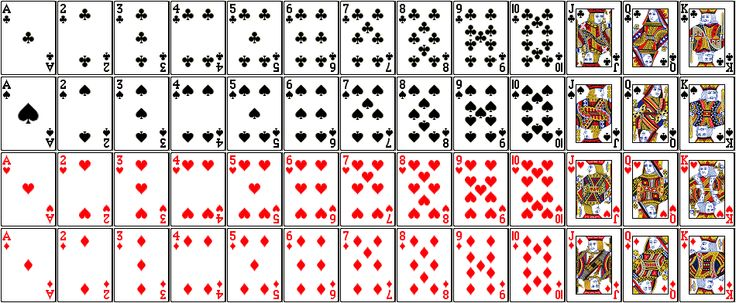
\includegraphics[width=10cm]{./pe/deck.jpg}
%  % deck.jpg: 0x0 pixel, 300dpi, 0.00x0.00 cm, bb=
%  \caption{Baraja inglesa}
%  \label{fig:deck}
% \end{figure}
%
% 
% [t]
%  \begin{exmp}
%   \label{solved:1.1}
%   Una carta se obtiene al azar de una baraja inglesa. Describa el espacio muestral si se consideran los palos.
%  \end{exmp}
%
% 
% {}
% Supongamos que $A$ es el evento \texttt{``se obtiene un rey''} o simplemente $\set{K},$ mientras que $B$ es \texttt{``se obtiene un tr\'ebol} o simplemente $\set{\clubsuit}.$
% 
% [t]{}
%  \begin{exmp}
%   \label{solved:1.2}
% % \begin{wrapfigure}{l}{5cm}
% % %%%%%%%%%%%%%%%%%%%%%%%%%%%%%%%%%%%%%%%%%%%%%%%%%%%%%%%%%%%%%%%%%%%%%%%%%%%%%%%%%%%%%%%
% % %%% You will need to add \usepackage{wrapfig} to your preamble to use textwrapping %%%
% % %%%%%%%%%%%%%%%%%%%%%%%%%%%%%%%%%%%%%%%%%%%%%%%%%%%%%%%%%%%%%%%%%%%%%%%%%%%%%%%%%%%%%%%
% %  \centering
% %  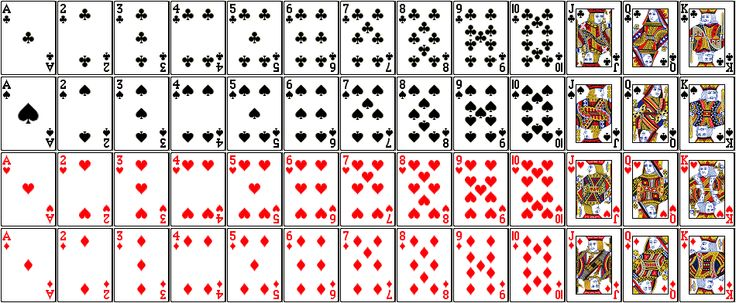
\includegraphics[width=5cm,keepaspectratio=true]{./pe/deck.jpg}
% %  % deck.jpg: 0x0 pixel, 300dpi, 0.00x0.00 cm, bb=
% % \end{wrapfigure}
% \begin{figure}
%  \centering
%  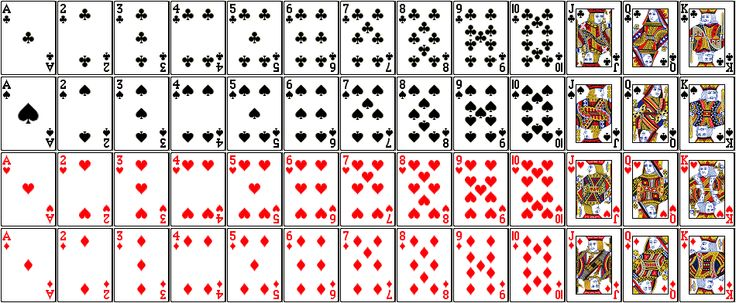
\includegraphics[width=9cm,keepaspectratio=true]{./pe/deck.jpg}
%  % deck.jpg: 0x0 pixel, 300dpi, 0.00x0.00 cm, bb=
% \end{figure}
% Sean $A=\set{K}, B=\set{\clubsuit}.$ Describa los siguiente eventos: 
% \begin{multicols}{2}
%  \begin{enumerate}[(a)]
%  \item $A\cup B$ 
%  \item $A\cap B$ 
%  \item $A \cup B'$ 
%  \item $A' \cup B'$ 
%  \item $A - B$ 
%  \item $A'-B'$ 
%  \item $(A\cap B) \cup (A\cap B')$
% \end{enumerate}
% \end{multicols}
%
%
%  \end{exmp}
% 
%
% [t]
%  \begin{exmp}
%   \label{solved:est.6.5}
%   De una baraja inglesa se extraen 2 cartas. Encuentre la probabilidad de que las dos sean ases si la primera carta
%   \begin{enumerate}[(a)]
%    \item se devuelve a la baraja 
%    \item no se devuelve a la baraja.
%   \end{enumerate}
%
%  \end{exmp}
%
% 
% [t]
%  \begin{exmp}
%   \label{solved:est.6.6}
%   En un contenedor hay 6 pelotas rojas, 4 blancas y 5 azules. Se extraen sucesivamente 3 pelotas. Encuéntrese la probabilidad de que se extraigan en el orden roja, blanca y azul si
%   \begin{enumerate}
%    \item cada pelota se devuelve a la caja 
%    \item no se devuelve.
%   \end{enumerate}
%
%  \end{exmp}
%
% 
% [t]
%  \begin{exmp}
%   \label{solved:est.6.7}
%   Encuéntrese la probabilidad de que en dos lanzamientos de un dado se obtengan por lo menos un 4.
%  \end{exmp}
%
% 
% [t]
%  \begin{exmp}
%   \label{solved:1.9}
%   Encuentre la probabilidad de no obtener 7 u 11 puntos en total al lanzar dos dados.
%  \end{exmp}
%
% 
% %%%
%
% \subsection{Probabilidad condicional}
{}
Sean $A,B$ dos eventos tales que $P(A)>0.$
\begin{figure}[h]
 \centering
 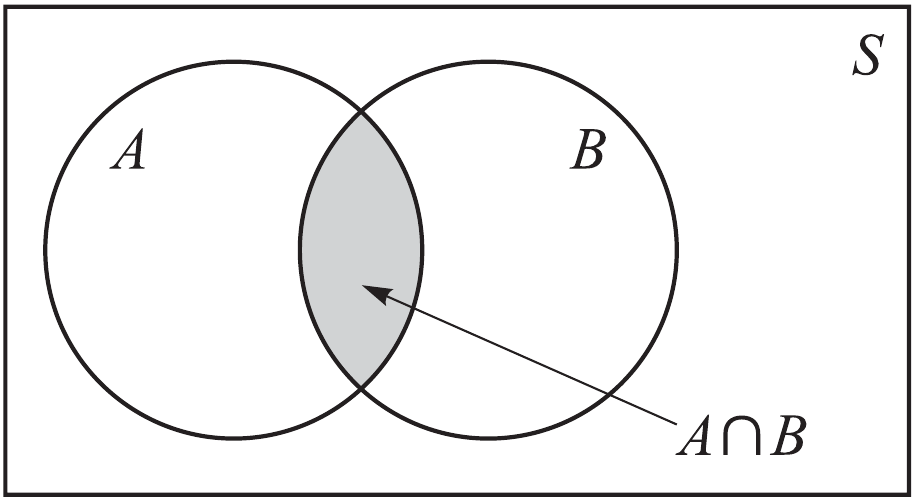
\includegraphics[width=5cm,keepaspectratio=true]{./pe/pands0103.png}
 % pands0103.png: 0x0 pixel, 300dpi, 0.00x0.00 cm, bb=
 \label{pands0103}
\end{figure}

  Denotaremos por $P(B|A)$
 la probabilidad de $B$ dado que $A$ haya ocurrido y diremos que es la \emph{probabilidad condicional} de $B$ dado $A.$
\section{Análisis combinatorio}

{}
El \emph{análisis combinatorio} es una manera sofisticada de contar.


\subsection{Principio fundamental del conteo y diagramas de árbol}

Si una tarea se puede realizar en $n$ formas diferentes y otra en $m$ formas diferentes, entonces las dos tareas se pueden realizar en $n\times m$ formas diferentes.


[t]{}
\begin{exmp}
	\label{exmp:1.14}
\end{exmp}
\begin{enumerate}
	\item Si una persona tiene 2 camisas y 4 corbatas, ?`de cuantas formas puede combinarlas?
	\item Construya un diagrama de árbol para representar todas estas opciones.
\end{enumerate}



\subsection{Permutaciones}
{}
Si tenemos $n$ objetos distintos y queremos ordenarlos tendremos
\begin{align*}
	n \times (n-1) \times ... 2\times 1
\end{align*} formas diferentes de hacerlo.

{}
\begin{defn}[$n$ factorial]
	\begin{equation}
		n! = \begin{cases}
			1 & n=0 \\
			n\times(n-1)! & n>0
		\end{cases}
	\end{equation}
	
\end{defn}


{}
Si tenemos $n$ objetos distintos y queremos arreglar $r$ de estos en una linea, entonces tendremos una \emph{permutación} de $n$ en $r$ dada por
\begin{align}
	\label{1.25}
	P^{n}_{r}=n\times(n-1)\times...\left( n-r+1 \right)
\end{align} 
o de manera equivalente
\begin{align}
	\label{1.27}
	P^{n}_{r}=\dfrac{n!}{(n-r)!}
\end{align}


[t]{}
\begin{exmp}
	\label{exmp:1.16}
	?`Cuantas permutaciones de longitud 3 se pueden formar con las letras $A,B,C,D,E,F,G$?
\end{exmp}


[t]{}
\begin{exmp}
	\label{exmp:1.17}
	Encuentre el número de permutaciones diferentes de las 11 letras de la palabra \emph{MISSISSIPPI}.
\end{exmp}


\subsection{Combinaciones}
{}
En una \emph{permutación}, uno está interesado en el orden de los objetos. Así $abc$ y $bca$ son permutaciones diferentes.  Pero en algunos problemas, uno está interesado sólo en elegir objetos sin importar su orden.  Tales selecciones se llaman \emph{combinaciones}.  Por ejemplo, $abc$ y $bca$ representan la misma combinación.



El número de combinación $ C^{n}_{r} $ al elegir $r$ objetos de una colección de $n$ diferentes está dada por el \emph{número combinatorio}
\begin{align}
	\label{1.29}
	C^{n}_{r} = \comb{n}{r}=\dfrac{n!}{r!\left( n-r \right)!}
\end{align}



{Algunas fórmulas combinatorias}
\begin{align}
	\label{1.30}
	\comb{n}{r}&=\dfrac{P(n,r)}{r!} \\
	\label{1.31}
	\comb{n}{r}&=\comb{n}{n-r}\\
	\comb{n}{r}&=\comb{n-1}{r-1}+\comb{n-1}{r}
\end{align}


[t]{}
\begin{exmp}
	\label{exmp:1.18}
	En una baraja inglesa, ?`cuantas formas hay de escoger dos cartas del mismo palo?
\end{exmp}


{}
\begin{thm}[Teorema del binomio]
	\begin{align}
		\label{1.32}
		\left( x+y \right)^{n} = \sum_{r=0}^{n}\comb{n}{r}x^{r}y^{n-r}
	\end{align}
	
\end{thm}


{Aproximación de Stirling}
\begin{align}
	\label{1.33}
	n! \approx \sqrt{2\pi n}\left( n^{n}e^{-n} \right)
\end{align}


% \subsection{Ejercicios resueltos}
% [t]{}
%  \begin{exmp}
%   \label{solved:1.22}
% 	Se requiere sentar a $5$ hombres y $4$ mujeres en una fila, de manera que estén alternados. ?`Cuantas manera hay de hacer tal arreglo?
%  \end{exmp}
% 
% [t]{}
%  \begin{exmp}
%   \label{solved:1.29}
% 	?`De cuantas manera podemos formar un equipo de 11 personas de un total de 23?
%  \end{exmp}
% 
% [t]{}
%  \begin{exmp}
%   \label{solved:1.35}
% 	Una caja contiene $8$ canicas rojas, $3$ blancas y $9$ azules. Si 3 canicas son obtenidas al azar sin reemplazarse, determine la probabilidad de que
% 	\begin{enumerate}[(a)]
% 	 \item las tres sean rojas; 
% 	 \item las tres sean blancas; 
% 	 \item dos sean rojas y una blanca; 
% 	 \item al menos una sea blanca; 
% 	 \item una sea de cada color; 
% 	 \item sean obtenidas en el siguiente orden: rojo, blanco y azul.
% 	\end{enumerate}
%
%  \end{exmp}
% 
% [t]{}
%  \begin{exmp}
%   \label{solved:1.36}
% 	En un juego de \emph{poker}, 5 cartas se obtienen al azar de una baraja inglesa. Encuentre la probabilidad de que
% 	\begin{enumerate}[(a)]
% 	 \item 4 sean $A$; 
% 	 \item 4 sean $A$ y una sea $K$; 
% 	 \item 3 sean $10$ y dos sean $J$; 
% 	 \item $9,10,J,Q,K$ en cualquier order; 
% 	 \item 3 de un palo dado y 2 de otro palo; 
% 	 \item al menos un $A$ obtenido.
% 	\end{enumerate}
%
%  \end{exmp}
% 
% [t]{}
%  \begin{exmp}
%   \label{solved:1.37}
% 		Determine la probabilidad de obtener tres $6$ en cinco lanzamientos de un dado.
%  \end{exmp}
% 
%


 \section{Probabilidad condicional}

 \subsection{Definición}

{}
\begin{defn}[Probabilidad condicional]
 \begin{align}
  P(B|A)&=\dfrac{P(A\cap B)}{P(A)} \\
  P(A\cap B) &= P(A)P(B|A)
 \end{align}
\end{defn}


{}
\begin{rem}
 La probabilidad condicional satisface todos los axiomas de una función de probabilidad.  Podemos pensar $P(\cdot|A)$ como la función de probabilidad que se obtiene al reemplazar el espacio muestral $S$ por $A.$
\end{rem}


[t]{}
\begin{exmp}
 \label{exmp:1.13}
 Encontrar la probabilidad de que una solo lanzamiento de un dado resulte en un número menor que $4$ si
 \begin{enumerate}[(a)]
  \item no hay más información; 
  \item se sabe que el lanzamiento resultó en un número impar.
 \end{enumerate}

\end{exmp}


\subsection{Teoremas sobre Probabilidad Condicional}
{}
\begin{thm}
 \label{thm:1.9}
 Para cualesquiera tres eventos $A_{1},A_{2},A_{3},$ tenemos que
 \begin{align}
  \label{1.19}
  P(A_{1} \cap A_{2} \cap A_{3})=P(A_{1})P(A_{2}|A_{1})P(A_{3}|A_{1} \cap A_{2})
 \end{align}
\end{thm}


{}
\begin{thm}
 \label{thm:1.10} Si $S=A_{1}\sqcup ... \sqcup A_{N},$  entonces
 \begin{align}
\label{1.20}
P(A)=P(A_{1})P(A|A_{1})+...+P(A_{N})P(A|A_{N})
\end{align}
\end{thm}


\subsection{Eventos independientes}
{}
Si $P(B|A)=P(B),$ i.e., la probabilidad de que $B$ ocurra no está afectada por la ocurrencia de $A,$ entonces diremos que $A$ y $B$ son independientes.


\begin{defn}
 $A$ y $B$ son eventos independientes si y solo si
 \begin{align}
  \label{1.21}
  P(A \cap B) = P(A)P(B).
 \end{align}
\end{defn}


{}
La definición se puede generalizar a más de dos eventos.  Por ejemplo, diremos que $A_{1},A_{2},A_{3}$ son eventos independientes si
\begin{align}
k\neq j \rightarrow P(A_{j} \cap A_{k})=P(A_{j})P(A_{k}), \; j,k=1,2,3 
\\ P(A_{1}\cap A_{2} \cap A_{3})=P(A_{1})P(A_{2})P(A_{3}).
\end{align}


{}
\begin{thm}[Teorema de Bayes]
 Si $S=A_{1}\sqcup A_{2} \sqcup...\sqcup A_{N},$ entonces
 \begin{align}
  \label{1.24}
  P(A_{k}|A) = \dfrac{P(A_{k})P(A|A_{k})}{\sum_{j} P(A_{j})P(A|A_{j})}
 \end{align}

\end{thm}



[t]
 \begin{exmp}
  \label{solved:1.16}
  Demuestre el teorema de Bayes.
 \end{exmp}



[t]{}
 \begin{exmp}
  \label{solved:1.15}
 La caja $I$ contiene 3 canicas rojas y 2 azules, mientras que la caja $II$ contiene $8$ canicas rojas y 8 azules. Una moneda se lanza: Si cae un sol, se escoge una moneda de la caja $I$ y si cae águila, de la caja $II.$ Encuentre la probabilidad de obtener una canica roja.
 \end{exmp}


[t]{}
 \begin{exmp}
  \label{solved:17}
	Supongamos que en el problema anterior, quien lanza la moneda no revela si ha caído águila o sol (de manera que la caja de la que se obtiene la canica no se revela) pero revela que una canica roja se ha obtenido.?`Cual es la probabilidad de haber obtenido un sol?
 \end{exmp}



